\chapter{Machine Learning}

As an introductory material, this chapter introduces what Machine Learning is and how it works. This chapter will illustrate the notions through the lens of activity recognition in images. However, the foundations laid out here are not limited to this use case and are indeed more general. The explanations will alternate between the specific use cases, to ease the intuitive understanding, and the more abstract concepts in order to make the generality of the techniques clear.

At the end of this chapter we will illustrate the foundations laid out here with a practical example. This will allow us to introduce the basics of model training, evaluation, data augmentation, and fine-tuning a pretrained model.

\section{What is Machine Learning}

\subsubsection{ML as functions}

Let $\mathcal{X}$ be the set of  images we are interested in, and $\mathcal{Y}$ be the set of activities. In order to solve the problem of activity recognition, we wish to find a function $f:\mathcal{X}\mapsto\mathcal{Y}$ that maps an image from $\mathcal{X}$ to its correct activity. 

While researchers have tried to write themselves algorithms that deciphers natural images, applications such as "search images by text" in Google Photos, image colorization, natural image generation or captioning remained out of reach. Indeed, researchers found more success writing algorithms that \emph{search} for $f$ rather than finding $f$ themselves. Image understanding is now dominated by \emph{machine learning} approaches, that is, algorithms finding $f$ from examples.

In fact, $\mathcal{X}$ does not have to be images, and $\mathcal{Y}$ class labels. As long as there is a relationship between $\mathcal{X}$ and $\mathcal{Y}$, the former can be considered a random variable and the later a dependent variable. Machine Learning is about getting better at a task (with respect to a chosen metric) based on experience (or "examples", or "training samples").

\subsubsection{Parameters and hyperparameters}

In machine learning, we distinguish two kinds of values: parameters and hyper-parameters.

The values or decisions that are searched during learning for representing $f$ are the \emph{parameters}. For neural networks (defined later) they could be the individual neurons' synapses values, or \emph{weights}.

Sometimes, there are configurations for those algorithms that cannot be learnt during training, like the number of neurons or layers, the maximum depth of a decision tree, which are the aforementioned \emph{hyperparameters}.

\subsubsection{Train, validation, and test datasets}

Let a dataset $\mathcal{D}_t={(x_0, y_0), ...(x_N, y_N)}$ where the $x_i \in \mathcal{X}$ are the images and the $y_i \in \mathcal{Y}$ are their class labels (most of the time provided by humans), usually an integer between 0 and $|\mathcal{Y}|-1$. Machine Learning (ML) aims to find a function $f$ that, based on the examples provided in $D_t$, can approximate a correct $f$. This is usually called \emph{training or learning a model}.

Unfortunately, those functions found by ML techniques build complex relations hard to interpret by humans, sometimes known to be coarse approximations. Deep Learning solutions, and sometimes classical ML solutions are often considered black box. If we were able to understand it or not use approximations, we would have probably been able to write the function in the first place. It is often not possible to verify that the model solves the task in a meaningful way by checking its inner workings. Checking a ML model usually involves having a second set of annotated data $\mathcal{D}_v$ and checking the performance (accuracy, for instance) on this set of data, called \emph{validation set}. We have to rely on the validation set performance in order to trust that if the model solves them, then it has found an appropriate solution.

Finally, there is another catch. Some algorithms need to be configured with some \emph{hyperparameters} before learning on the training set. However, throughout a project's life, the model and algorithms evolve during development. In order to make sure those hyperparameters and this exact algorithm generalize well and are not just conveniently working for this validation set, there is usually a third set, the \emph{validation set} that is used in place of the test set during both development and hyperparameters selection. The test set $\mathcal{D}_e$ is used as little as possible, only when trying to have a clear evaluation of the performance of the model. The test set, in order to be predictive of the model's final performance, should be representative of the real world data.

Every time the developer or the learning algorithm tunes parameters or hyperparameters, there is a risk that they become tailored to this dataset exactly. This is called overfitting: decreasing generalization and improving the performance on the training set. The test set exists to test whether the learning algorithm overfitted parameters on the training set.

The developer adjusts various hyperparameters (model size, learning rate, etc) in order to maximize the performance on the validation set. In order to make sure that those hyperparameters decisions generalize beyond the test set, we need a third set, the validation set. Unfortunately, as we use more and more the validation set to test various models, there is a risk of overffiting it as well.

Indeed, some datasets are used so commonly by researchers that there is a risk that the models and algorithms tested on those don't generalize as well and are accidentally tuned to those datasets specifically \citep{imagenetgeneralizeimagenet}.


\section{Neural Networks}

\subsection{Neural Networks in computer vision}

While there are many algorithms that are able to learn from examples, computer vision is nowadays largely dominated by neural networks. They gained a lot of traction in 2012 when the ImageNet challenge \citep{imagenet} was won by a large margin with neural networks \citep{alexnet} rather than classical image processing techniques using classical machine learning (kNN, SVM, decision trees, etc \citep{bishop}). The next year, in 2013, all competitors used neural networks. In 2015, they started gaining traction in the industry as well. I can remember, that year, when interning in Google, Sundar Pichai pitching Google Photos and explaining how big resnets \citep{resnet} made it possible, less than a full year after their discovery.

\subsection{Neurons}

\begin{figure}[h]
    \centering
    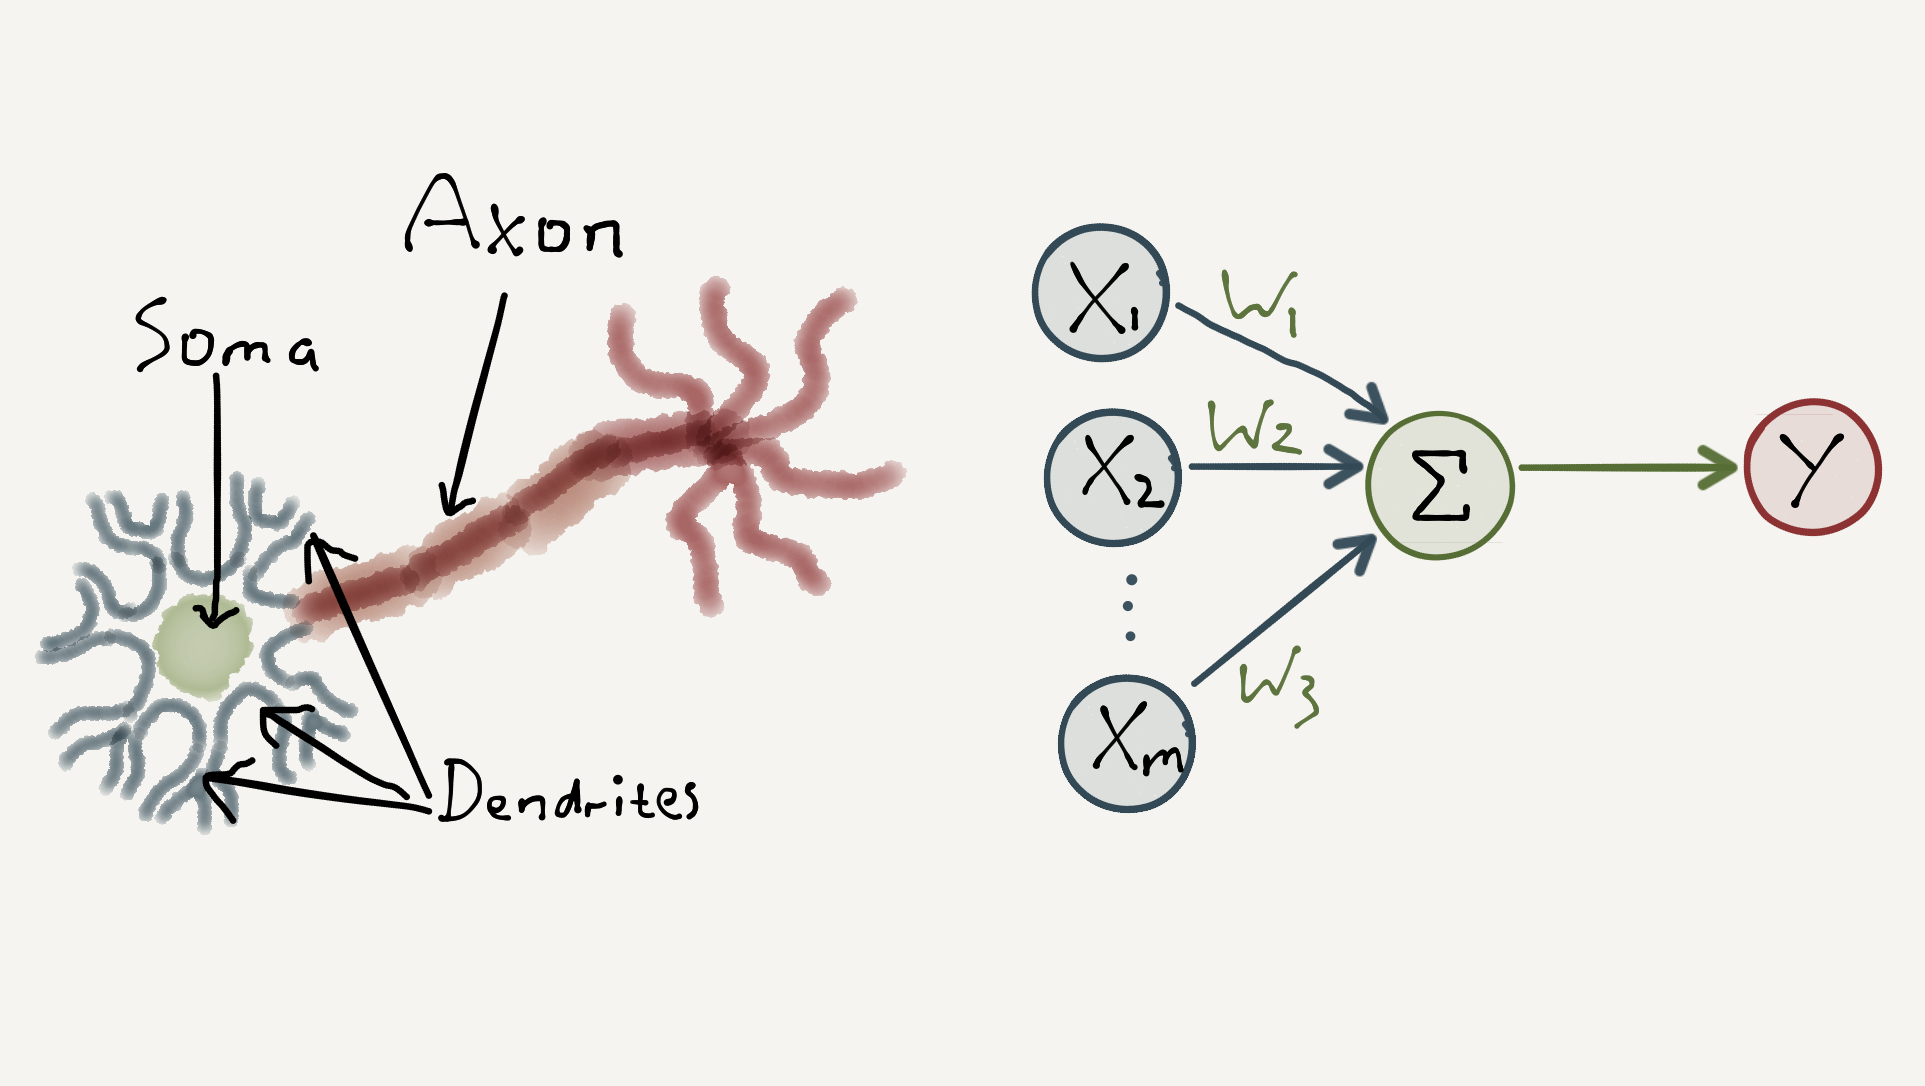
\includegraphics[scale=0.1]{30-activity/neuron.png}
    \caption{A (very simplified) biological neuron and an artificial neuron (Perceptron)}
    \label{fig:neuron}
\end{figure}

Before understanding neural networks, let's focus on a single artificial neuron. Artificial neurons are loosely inspired by biological neurons. They represent a neuron taking some input electrical signals, transmitting those by weaker or stronger dendrites (connections), summed up in the soma, firing through the axon if the total amount is above a certain threshold. Cf Figure \ref{fig:neuron}

In computer science, this is approximated by a linear combination $\textbf{w}$ - a weighted sum - of the input $\textbf{x}$, followed by a threshold $b$ and an activation function $\sigma$. An artificial neuron is then $\sigma(\textbf{w}^T\textbf{x}+b)$, with $\sigma$ being any non-linear function. \emph{Training a neuron is finding the weights $\textbf{w}$, $\textbf{b}$ that works best for solving a given problem}. This is sometimes still called a Perceptron, in reference to the original paper by \citet{perceptron}.

While today we often chose the \emph{Rectified Linear Unit} (ReLU) $\sigma(x)=\max(0, x)$ for its good numerical and computational properties \citep{relu}, researchers initially used a sigmoid, tanh or step function. Developing on activation functions is well beyond the scope of this manuscript, but it is still an active area of research with new propositions, despite none of them outperforming the performance / computational cost tradeoff of ReLUs.

\subsection{From single neurons to neural networks}

Once we have a neuron, there are two ways we can add more to build a \emph{neural network}: either by parallel neurons (the \emph{width}) or by stacking them in successive \emph{layers} (the \emph{depth}). The Universal Approximation Theorem \citep{universalapprox} states that a neural network with 2 layers and enough neurons \cite{mlpbounds} can theoretically approximate any computable function. Unfortunately, possible does not equate practically feasible and we needed decades before turning them into useful algorithms. The deception lies in the "enough" part, which can be intractable for any practical purpose.

Fortunately, it has been shown that width can be traded with depth \cite{widthdepth}, allowing neural networks to work in successive abstractions \citep{deepbelief,deepviz}, thus not needing stellar amount of data and compute. Deepening neural networks was not possible immediately, and required new tools (among which the aforementionned ReLU), explaning why neural nets remained shallow for so long.

\subsection{Training neural networks}

\begin{figure}
    \centering
    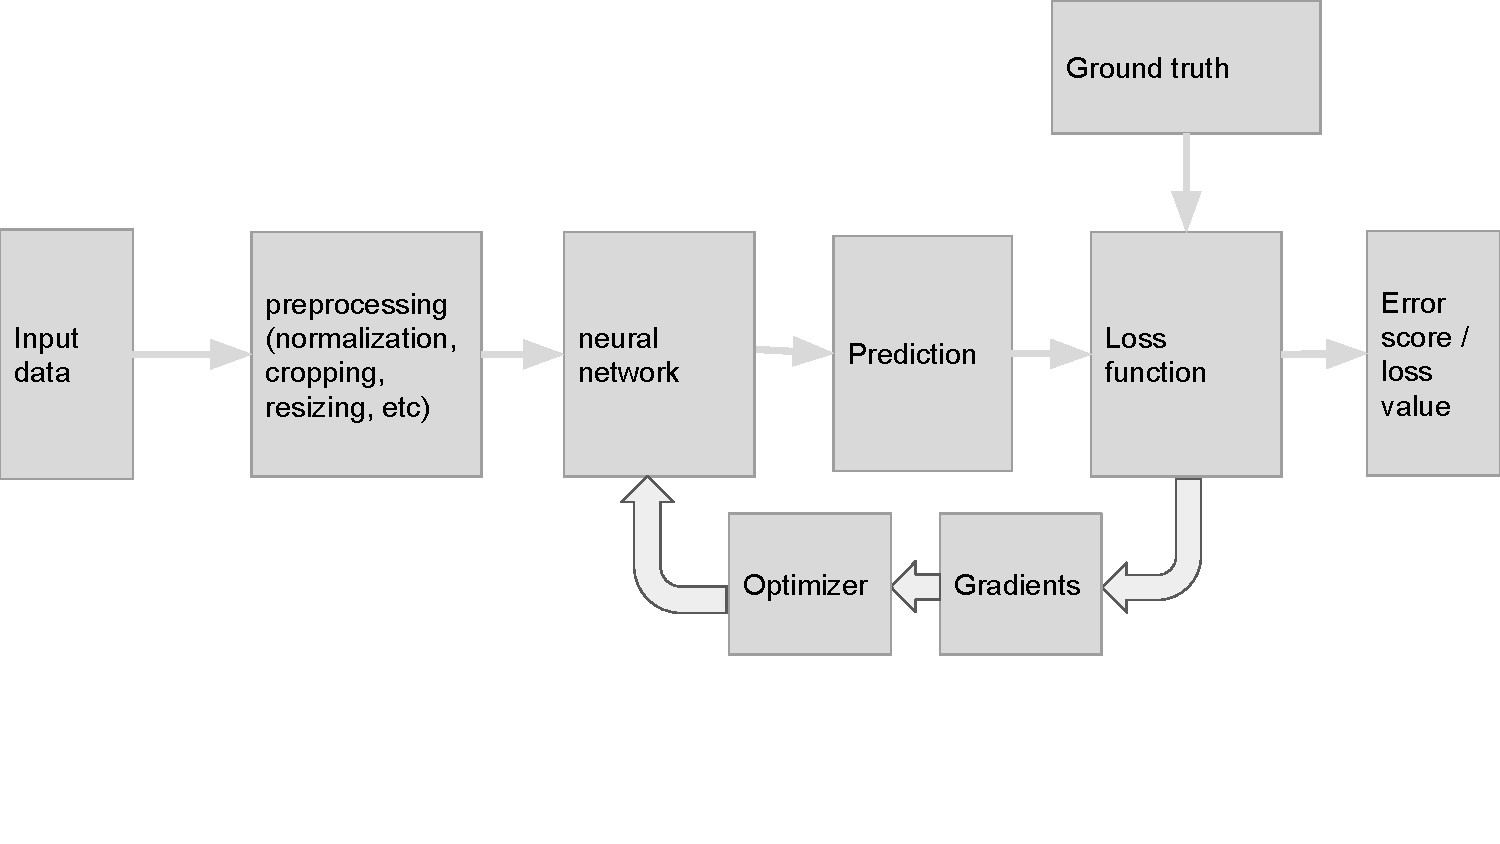
\includegraphics[width=\columnwidth]{30-activity/workflow.pdf}
    \caption{A neural network training loop}
    \label{fig:trainingloop}
\end{figure}

After describing what neural networks \emph{are}, it is necessary to describe how they \emph{work}. Neural networks are stacks of non-linear layers, composed of many tunable weights $\theta$ computing data transforms. How do we train them?

Neural Networks are built from differentiable components, making $f_\theta(\cdot)$, the function they compute, differentiable as well. In the simplest case, the training dataset provides an input $x$ and expected correct answer $y$. We compute $\hat{y}=f(x)$, the maximum likelihood answer given by the network. Then, a differentiable predefined function $\mathcal{L}(\hat{y}, y)$ computes the distance between the generated answer and the expected correct answer. By differentiating this distance wrt to the parameters $\theta$, we get the direction in which to move $\theta$ to reduce the error. $\theta$ is moved a bit (a step of size $\alpha$) in this direction and the iterative process continues, and $f$ learns to provide better and better answers. This process is called \emph{Gradient Descent}. In Deep Learning, however, \emph{Stochastic Gradient Descent} (SGD) is used. The stochasticity comes from the fact that we compute the gradient on a random subset of the dataset (a \emph{batch} or minibatch), each iteration. This helps regularizing the model (thus providing greater generalization), and descending on the full dataset is often not practically doable anyway since they are usually too big to fit in memory along with the gradient information. Each iteration thus fundamentally computes

\begin{equation}
    \theta := \theta - \alpha \nabla_\theta \mathcal{L}(f_\theta(x), y)
\end{equation}

However, as we will later see, this update equation can be made more sophisticated in order to reduce the number of steps needed to converge and / or improve generalization. These approaches are called \emph{optimizers}.

This process is summarized in Figure \ref{fig:trainingloop}.

\subsection{Data Augmentation}
\label{sec:trivialaugment}

Last but not least, neural networks have the capacity to fit and memorize even big datasets. When the networks start to memorize the training set, the model overfits and its generalization abilities decrease. One way to fight against that overfitting is to add more training data, but this is often expensive or hard. Instead, one can create artificial new examples by modifying the training set. For images, this can be flipping the pictures, rotating them, changing the illumination, etc. This also injects domain knowledge into the algorithm about the existing invariances. This is called \emph{data augmentation}. Tremendous progress has been made thanks to augmentation strategies \citep{cutmix,randaugment,mixup}. Examples from AutoAugment from \citet{autoaugment} are shown in Figure \ref{fig:autoaugment}.

\begin{figure}
    \centering
    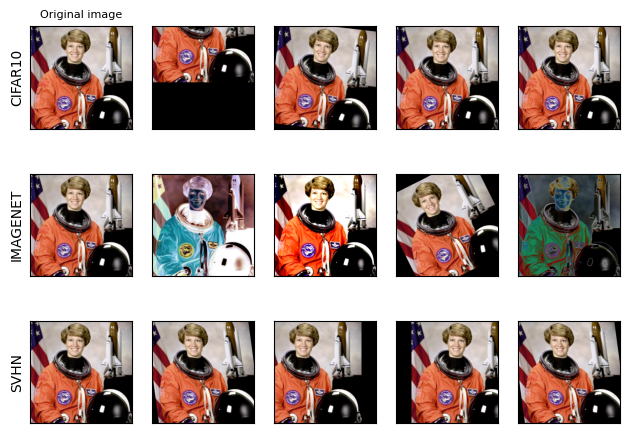
\includegraphics[width=\columnwidth]{70-files/autoaugment.png}
    \caption{Example of data augmentation. The original image is transformed to artificially generate new training examples. In this case, AutoAugment is used ; it combines multiple transformations and its settings depend on the dataset and the task. Figure from torchvision's documentation. Each row shows the set of augment used for those datasets on a sample image.}
    \label{fig:autoaugment}
\end{figure}

In this work, we will mainly use TrivialAugment \cite{trivialaugment}. It is a recent and very simple augmentation algorithm from which we can learn that despite a lot of complicated methods to automatically find augmentation policies (AutoAugment \cite{autoaugment}, RandAugment \cite{randaugment}, ...), yet the simplest method performs comparably or better.

TrivialAugment defines an augmentation as "a function a mapping an image x and a discrete strength parameter m to an augmented image". It uses a collection of predefined classic image transformations (color, contrast, rotation, ...). It randomly selects one of this operation per sample, and randomly sample its strength parameter m.

\subsection{Architecture}

What those layers of neurons compute and how they are arranged define an \emph{architecture} or \emph{topology}.

When two or more Perceptrons layers are stacked, it is called a \ac{MLP}.

However, Perceptrons do not perform well on natural image data. They are too general and somehow too powerful for computer vision: a Perceptron treats each and every input as separate variables, but pixels values are not independant variables. First, they are spatially correlated as the world is compositional, and exhibits many invariances in translation, scale, and orientation.

Perceptrons have to learn to perform the same operations everywhere on the picture, and, in practice they don't. Replacing Perceptrons with convolutions with learnable weights gave birth to \acp{CNN}.

A convolutional layer is a Perceptron in disguise. It is just applied repeatedly and similarly on smalls spatial patches of the input. The size of that input patch is called \emph{kernel size}. We compute many different convolutions on the same input - the \emph{width} of the convolutional layer. Perceptrons compute multiple different linear combinations of the input in the same way -, each resulting spatial map is called a \emph{feature map} or \emph{channel}. Finally, the convolution kernel can jump some inputs, we call this \emph{strided} convolutions, in order to downsample the input resolution.

Convolutions instead of Perceptrons builds into the model what are called \emph{inductive biases}: they perform local operations - addressing compositionality - and performs them the same way everywhere on the picture - addressing translational invariance -. \acp{CNN} got fame in 2012 when they beat their competitors in the ImageNet classification challenge by a large margin and created the deep learning hype we know today \citep{alexnet}.

\begin{figure}
    \centering
    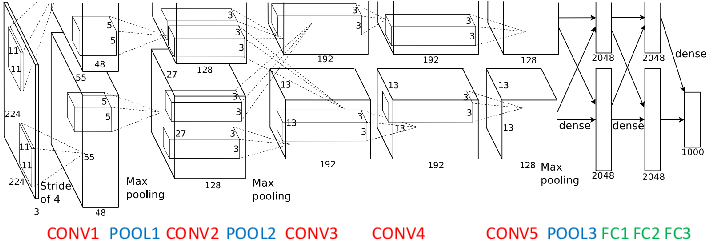
\includegraphics[scale=0.5]{30-activity/AlexNet.png}
    \caption{AlexNet architecture, built from convolutions (CONV), pooling operations (POOL), and linear layers (FC). Figure from \citet{alexnet}}
    \label{fig:alexnet}
\end{figure}

The convnet that made deep learning attractive by winning ImageNet is \textbf{AlexNet} \citep{alexnet} (see Figure \ref{fig:alexnet}). It contains 5 conv layers, 2 max pooling layers, and 3 linear layers (also called Fully Connected layers). Max Pooling are meant to reduce the spatial size in order to reduce both memory and compute consumption, and increase the working region of each convolution. As the image is processed through the convnet, it produces layers of activations, that gets abstracted in neural representations. Deep representations have a low spatial resolution but rich semantics \citep{deepbelief,deepviz}.

\begin{figure}
    \centering
    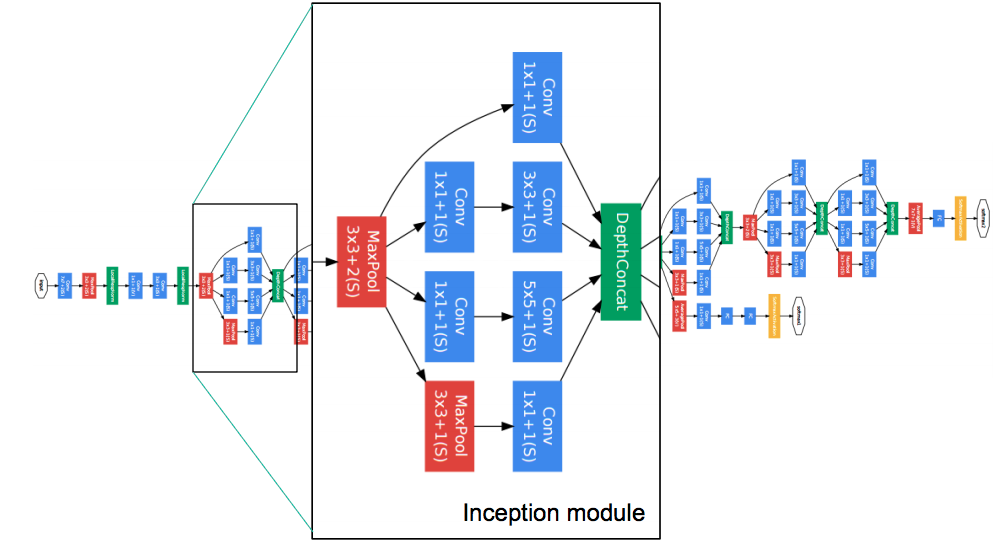
\includegraphics[width=\columnwidth]{30-activity/googlenet.png}
    \caption{GoogLeNet / Inception-v1. It uses complex building blocks, aggregating different design decisions. Figure from \url{https://medium.com/@RaghavPrabhu/cnn-architectures-lenet-alexnet-vgg-googlenet-and-resnet-7c81c017b848}}
    \label{fig:googlenet}
\end{figure}

The design of convnets raises many questions: how many channels? what kernel shape? what stride? Should we pool? It is hard to answer those, so, when designing \textbf{GoogLeNet} / \textbf{Inception} \citep{googlenet} (Cf Figure \ref{fig:googlenet}), the Google team stacked many layers of complex building blocks. Each of those blocks is composed of parallel paths taking different design decisions. At train time, the net can learn to use each of those paths to its best.

\begin{figure}
    \centering
    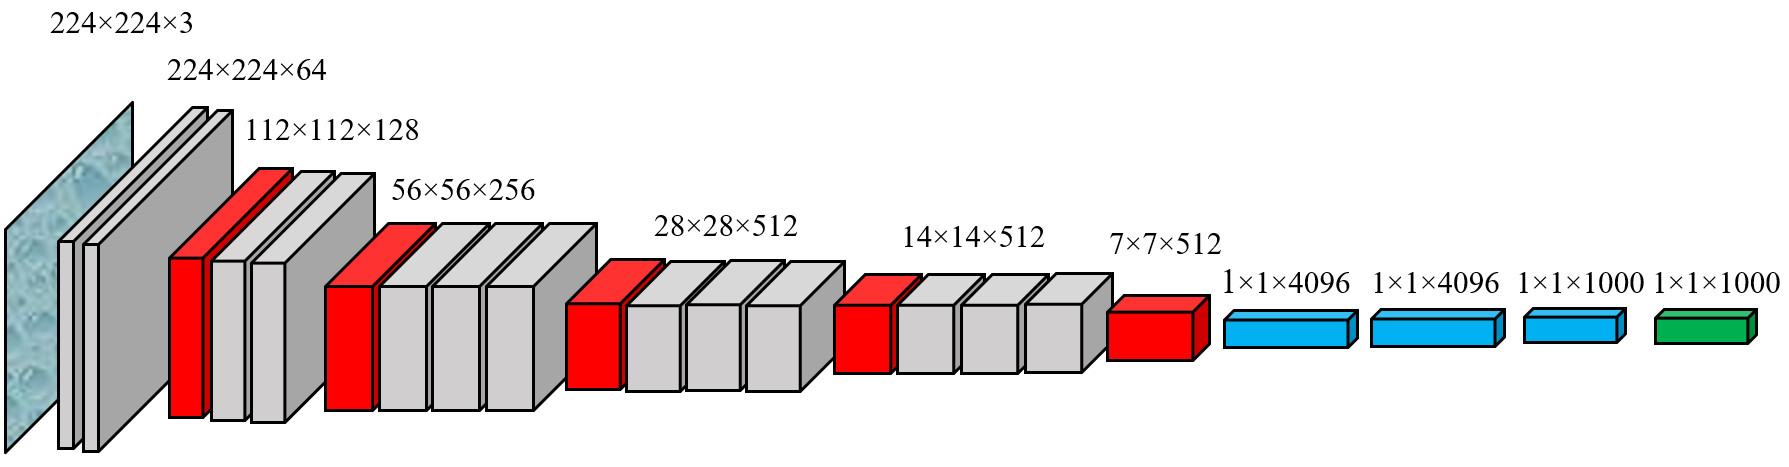
\includegraphics[width=\columnwidth]{30-activity/VGG_neural_network.png}
    \caption{VGG network. Grey: 3x3 convolution layers; red: pooling layers; blue: linear (or 1x1 convs) layers; green: softmax}. Each activation is described as $\text{Heigth} \times \text{Width} \times \text{Channels}$.
    \label{fig:vgg}
\end{figure}

However, those questions might not be that important after all. The \textbf{VGG} net  \citep{vgg} (Cf Figure \ref{fig:vgg}) uses only 3x3 convolutions, and doubles the number of channels after each pooling operation. Its simplicity encouraged researchers to invest time into simple designs with better fundamental principles rather that complex models.

\begin{figure}
    \centering
    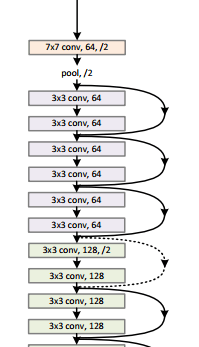
\includegraphics{30-activity/resnet.png}
    \caption{In ResNets, an identity path is added, so that the gradient can flow up to the first layers untouched. Figure from \cite{resnet}}
    \label{fig:resnet}
\end{figure}

\citet{resnet} observed that VGG nets could not be made very deep (no more than 20 layers). They hypothesized that the gradients quickly lose their supervision quality going back through the layers, failing to update the first layers. From this, they chose to design \emph{residual} networks, where convs compute additive residual transformations. The gradients can then flow unchanged along the identity path and keep its informative quality. The \textbf{Residual Network} (ResNet, cf Figure \ref{fig:resnet}) can go at least up to 1000 layers and still learn, despite reaching diminishing returns after 150 layers. The 50 layers variant is the most widely used because of its compute cost / performance tradeoff. ResNets were such an improvement that most of the following architectures integrated residual connections.

Note: Perceptrons are making their great comeback in image processing \citep{mlpmixer}, mostly through Transformers (Perceptrons with an attention mechanism) \citep{transformers,vit}. However, it does not invalidate what was said previously: while their performance scale better wrt big data quantity than \ac{SotA} \acp{CNN}, they perform worse than \acp{CNN} on smaller training sets (ImageNet-1k being considered "small" in this context). Indeed, despite limiting convnets at scale, the convolutional inductive biases embody some knowledge about natural images. Transformers based architectures need some more data to discover those invariances and close the gap, but are able to surpass \acp{CNN} with even more data. There are works trying to suggest inductive biases to vision transformers that the network can un-learn if needed, in order to make them perform on par or better than convnets in lower data regimes \citep{convit,coatnet} and always benefit from their scalability.

\subsection{Optimizers for Deep Learning}

Developing on optimizers is way beyond the scope of this work, but they cannot be kept unspoken of either. We briefly mention the main optimizers used for training deep networks.

\subsubsection{Stochastic Gradient Descent}

When gradient descent is done on a random subset of the training data, it becomes \ac{SGD}. \ac{SGD} is akin to walking the steepest direction in a valley in order to reach a minimum.

\ac{SGD} is slow and prone to underfitting as it has no mechanism to escape small local minima.

For weights $\theta$, gradient of the loss $\nabla J$, and hyperparameter learning rate $\alpha$:

\begin{equation}
    \theta := \theta - \alpha \nabla J
\end{equation}

\subsubsection{Stochastic Gradient Descent with Momentum}

Instead, \ac{SGD} is almost always used in its momentum variant. Taking the same analogy, \ac{SGDM} is like \emph{rolling} in the steepest direction. While we roll, we accumulate velocity $v$ that might help escape small local minima. Even if the valley is irregular, momentum helps escape those irregularities and reach the bottom. It adds a new momentum hyperparameter $\beta$.

\begin{equation}
\begin{split}
    v := & v + \beta \nabla J \\
    \theta := & \theta - \alpha v
\end{split}
\end{equation}

Another notable variant is Nesterov momentum. Here, the gradient evaluation is performed after the momentum step of the parameters, contrarily to SGDM.

\subsubsection{Adam}

Another family of optimizers, the \emph{adaptive optimizers}, made popular by \emph{\ac{Adam}} is said to be less sensitive to hyperparameters and especially to the learning rate. It works by scaling the learning rate by the rolling variance of the weight in the recent history. It introduces new hyperparameters, $\beta_1$ and $\beta_2$, respectively defaulted to 0.9 and 0.999. It also considers $t$, the number of the current iteration, and $\epsilon$, a constant for numerical stability.

\begin{equation}
\begin{split}
    m := & \beta_1 m + (1 - \beta_1) \nabla J \\
    v := & \beta_2 v + (1 - \beta_2) \nabla J \\
    \hat{m} := & m / (1 - \beta_1^t) \\
    \hat{v} := & v / (1 - \beta_2^t) \\
    \theta := & \theta - \alpha \hat{m} / \sqrt{\hat{v} + \epsilon}
\end{split}
\end{equation}

Despite its advantages in convergence speed and hyperparameters tuning, it has not fully took precedence over SGD as it converges to results only close to SGDM performance.

The literature explored many variants, including AdamW, RAdam, AdaMax, AMSGrad, AdaBelief, etc.

\subsection{Loss functions}

Any differentiable function that measures the error of the prediction can be used as a loss function. We will quickly lay out the most commonly used functions. 

\subsubsection{Cross-Entropy}

Cross-Entropy is used when the predictions are interpreted as the parameters of a categorical probability distribution. Cross-entropy measures the difference between two categorical distributions: the predicted distribution $p$ and the target distribution $\hat{y}$.

\begin{equation}
    \mathcal{L}(p, \hat{y}) = - \sum_i \hat{y}_i \log p_i
\end{equation}

In order to train a classifier, it optimizes the network's weights to predict a probability of 1 in the target class, reducing the other probabilities towards 0. This is strictly equivalent to maximizing the probability of the target class, or minimizing the negative log likelihood of the target class. The later formulation is preferred as it is computationally cheaper.

A neural network does not produce calibrated probability distributions on its own, but unconstrained scalars. They are often called \emph{logits}, as unnormalized log parameters of the categorical distribution, interpreted as the output of the logit function. Those logits $z_i$ can be be normalized into the categorical distribution parameters $o$ with the softmax function.

\begin{equation}
    o_i = \frac{\exp (z_i \tau)}{\sum_j \exp (z_j \tau)}
\end{equation}

Where $\tau$ is an optional \emph{temperature} parameter that controls the sharpness / entropy of the distribution.

While not being totally accurate, some people call the cross-entropy loss \emph{softmax loss}.

\subsubsection{Mean-Squared Error}

When trying to predict continuous values, one's default loss function choice is the L2 distance, or \ac{MSE}

\begin{equation}
    \mathcal{L}(y, \hat{y}) = (\hat{y}_i - y_i)^2
\end{equation}

\paragraph{Note: Numerical Considerations} When working with probabilities, computers might run into issues. Probabilities $p_i$ are often multiplied together and can become small, to the point where there could be representation issues with standard IEEE754 32 bits floats. For this reason, when possible, we instead manipulate log probabilities, taking advantage of this property:

\begin{equation}
    \prod_i p_i = \exp \sum_i \log p_i
\end{equation}

\subsection{Common datasets}

Some datasets are commonly used in computer vision in order to develop new techniques, compare models, or leverage knowledge from big datasets.

\subsubsection{MNIST}

MNIST \citep{mnist} is dataset of 28x28 greyscale images representing handwritten digits labeled with the ground truth digit. It contains 60k training pictures and 10k testing pictures. Classifying those digits is such a simple task that a SVM reaches 0.8\% error. In deep learning, MNIST is used as a sanity check for debugging or to introduce novel ideas, for instance with artificially introduced label noise.

\subsubsection{CIFAR-10/100}
\label{cifar10}

CIFAR-10 \citep{cifar10} contains 50k training 32x32 color images of 10 classes (airplane, automobile, bird, cat, deer, dog, frog, horse, ship, truck). There are 10k test images. This dataset is often used for developing new strategies. Optimizers, architectures, augmentations etc are often tested and calibrated on CIFAR-10 before before being battle-tested on ImageNet.

CIFAR-100 is similar but extended to 100 classes, 600 images each. It is not as commonly used as CIFAR-10.

\subsubsection{ImageNet-1K / ILSVRC12}

ImageNet (sometimes called ILSVRC for Image Large-Scale Visual Recognition Challenge) \citep{ILSVRC15,imagenet} is a large scale database of natural images crawled from the web, divided into 1k classes. It contains about 1M training pictures (~1k per class) and 50k testing images.

Since 2012, ImageNet has been the gold standard dataset for evaluation and comparison of classifiers. It is also commonly used to extract knowledge from natural images in order to build feature extractors or backbones for assembling models together \citep{imagenettransfer}. An expanded version of ImageNet, ImageNet-21k has been released. Models able to ingest lots of data are usually pretrained on it, before being tested on ImageNet-1k.

\section{\emph{\arr Practical Example}: A classifier for HActions}
\label{actionclf}

In this section we show how a standard image recognition problems can be solved with the tools laid out in this chapter. This is illustrated on activity recognition on the HActions dataset.

Activity recognition aims to identify what people are doing in still pictures or videos. At Hexaglobe, we are interested in activity tags in order to add metadata to our customers' content. They can be fed to search engines and recommender systems for more relevant results, as well as explicit categorization for a better user experience.

Most of the time, a still picture is enough to infer the activity: people sitting at a table with food are likely eating, people holding a microphone are most probably singing, etc.

\subsection{The model}

For industrial settings such as this one, training speed is more important than accuracy, so the tradeoff should favor iterative development. For this reason, I chose a ResNet-18 as our network. It has less parameters (11M) than the popular ResNet-50 (24M) for the sacrifice of few accuracy points.

As the HActions dataset (see section \ref{sec:hactions}) at most 2400 examples per class, training a model from scratch is likely to be suboptimal. In those situations where the dataset is relatively small, it helps to use \emph{transfer learning}. I chose to leverage a ResNet-18 from torchvision, pretrained on ImageNet-1k. The fact that both datasets are made of natural images suggests that the pretrained knowledge will be useful.


\subsection{Transfer Learning}

Natural images share common properties: neighboring pixels are correlated, the distribution of colors and brightness is not uniform, and some shapes occur frequently. When training a model on a large dataset such as ImageNet, the model would learn generic patterns, filters, shapes or objects that would be useful for other datasets or other tasks as well.

The parameters and architecture of the net is then kept untouched (or "frozen") but the last layer(s) that are trained on the new task. The frozen layers are used as a fixed feature extractor. This way, we only learn a small model from semantically rich features, instead of a bigger model from raw pixels. This allows to reuse natural images knowledge extracted from ImageNet. It helps preventing overfitting on meaningless spurious patterns in the case of small training sets, and to reuse knowledge for a different task. In addition to the performance advantage, this is much faster than training the whole thing as the features can be pre-computed only once.

After these last layer(s) have been retrained, it sometimes helps to \emph{fine tune} all the parameters of the model, by iterating a little more on the dataset, this time training the whole network with a very small learning rate. This allows the model to extract a few more useful or specific features that were not learned during the pretraining, while trying not to overfit . When possible, it helps to know how the base network has been trained as regularizers can improve ImageNet accuracy but reduce transferability \citep{imagenettransfer,crossentropytransfer}.

\subsection{Experiments}

\begin{table}[]
    \centering
    \begin{tabular}{|l|c|}
    \hline
        \textbf{Config} & \textbf{Test accuracy (\%)} \\
    \hline
        A: from random weights & 37.82 \\
    \hline
        C1: A + random flip & 43.87 (+10.05)\\
    \hline
        B: pretrained weights & 52.44 (+14.62) \\
    \hline
        C2: B + random flip & 55.67 (+3.23) \\
    \hline
        D: C2 + random crop & 55.67 (+0) \\
    \hline
        E: D + TrivialAugment & \textbf{58.19 (+ 2.52)} \\
    \hline
    \end{tabular}
    \caption{Test accuracy on HActions according to various configurations}
    \label{tab:hactivity_results}
\end{table}

In order to demonstrate what we laid down so far we run a quick set of typical experiments with a ResNet-18. All experiments are conducted with SGDM, weight decay (regularizing the square of the weights) is set to 1e-3, momentum is set to 0.9, batch size to 128, split across 4 GPUs. The learning rate is searched in \{0.3, 0.1, 0.01, 0.001, 0.0001\}. We train for 40 epochs. The \ac{lr} decays linearly from its initial value to 0 at the end of the training as \citep{lineardecay} shows this to be a sensible choice in common scenarios. The initial data augmentation includes random horizontal flipping and the pictures are resized to 128x227 which is unusual but keeps the 16:9 aspect ratio of the frames. We use a standard cross-entropy loss. A run takes about 1h.

We wish to verify and exemplify the benefits of a pretrained model and data augmentation, known to be among the top strategies to improve a natural images classifier.

The results, summarized in Table \ref{tab:hactivity_results}, show the power of pretraining and data augmentation, allowing performance boost with fast experiments. 

\paragraph{Config-A} trains from scratch. The best learning rate found is 0.1. It reaches an accuracy of 37.82\%.

\paragraph{Config-B} verifies that weights pretrained on ImageNet actually boost the accuracy. All the BatchNorm layers are kept in inference mode during training and the running statistics are not updated. The learning rate for all the layers but the last is set to 0 during the first 4 epochs and divided by 100 for the following iterations. The best learning rate found is 0.01. This significantly boosts the accuracy by 15\%, reaching 52.44\%.

\paragraph{Config-C} Config B is found to perform significantly better than A. Config-C adds random horizontal flipping of input images. Adding this transformation brings the random initialization (C1) to 43.87\%, and Config-B to 55.67\% (C2).

\paragraph{Config-D} adds inception-style random cropping to Config-C. It crops a random area from 80\% to 100\% of the image and resizes it to the input size.

\paragraph{Config-E} adds TrivialAugment (Section \ref{sec:trivialaugment}). The accuracy moves up to 58.19\%.

\subsection{Results and interpretation}

We trained a standard modern activity classifier from still pictures on HActions. Although 58\% may seem low, the dataset happens to be fairly small for classes that are loosely defined and somehow semantically hard to distinguish. For instance, if we were to classify dance move frames, the first and last few frames of each move, when the move starts and ends and is not clearly identifiable, this can legitimately be confused with no move at all. Upon manual inspection of the prediction on the test set, we indeed find that most of the errors can be attributed to ambiguity. The remaining errors can be largely attributed to a lack of data as they exhibit patterns not covered in training.

We would certainly solve many of those uncertainties by analyzing videos and neighbouring frames instead of independent frames, but that would come at a prohibitive cost. Instead we will consider those samples from a label noise perspective, hoping to construct a dataset without confusing training samples and reject ambiguous samples at inference time.

\section{Conclusion}

We demonstrated how the building blocks explained in this chapter (Figure \ref{fig:trainingloop}) can be assembled in order to train and utilize a learning algorithm. Pre-trained models for most used classification models are readily available and the data augmentation strategies are based on simple image manipulations. We show how one can leverage those for quick starting a project with little compute and data.

We trained a standard modern deep image classifier, leveraging battle tested techniques. Yet, the accuracy we obtained are usable for our use case, but somewhat below what can be expected from ImageNet capable models. We are facing problems that arise with "real world" usages: low data availability, labeling cost, ambiguity in samples and class semantics, etc. For instance, while ImageNet is a dataset of natural images, there are some peculiarities that might not be considered "real world", notably the data collection protocol that biased the data (keywords from search engines), or the fact that the class is an object centered and occupying the majority of the image surface.

In the next chapters, we apply the same standard classifier to the problem of face recognition, but quickly observe the same phenomenon: some data dependent problems are starting to arise, and need mitigation: there are some specific types of label errors that need to be fixed, the face extraction pipeline sometimes extracts non-face images, and the data bears its own set of hard features (very narrow demographics, extreme facial expressions, varying makeup, etc). The next chapter investigates dealing with label noise so as to mitigate the most damaging aspect of our training set: erroneous training samples.